\documentclass{article}
\usepackage{amsmath}
\usepackage{tikz}
\usetikzlibrary{angles, quotes}

\begin{document}

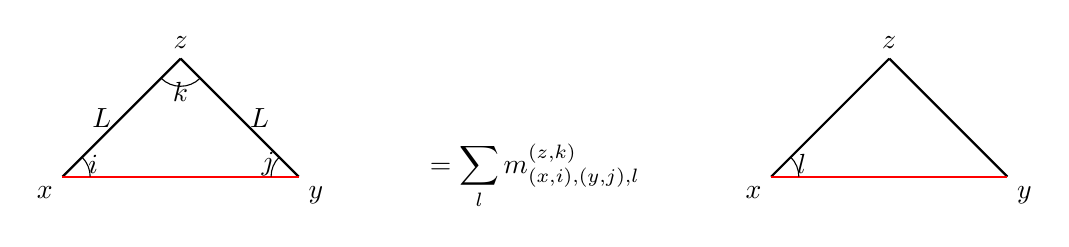
\begin{tikzpicture}[scale=1.5]

% Left diagram
\begin{scope}[shift={(-3,0)}]
    % Define coordinates
    \coordinate (A) at (-1,0);
    \coordinate (B) at (0,1);
    \coordinate (C) at (1,0);

    % Draw lines
    \draw[thick] (A) -- (B) node[midway, left] {$L$};
    \draw[thick] (B) -- (C) node[midway, right] {$L$};
    \draw[thick, red] (A) -- (C);

    % Mark angles
    \pic[draw, angle radius=10pt, "$i$", angle eccentricity=1.2] {angle = C--A--B};
    \pic[draw, angle radius=10pt, "$j$", angle eccentricity=1.2] {angle = B--C--A};
    \pic[draw, angle radius=10pt, "$k$", angle eccentricity=1.2] {angle = A--B--C};

    % Add labels
    \node at (A) [below left] {$x$};
    \node at (B) [above] {$z$};
    \node at (C) [below right] {$y$};
\end{scope}

% Right diagram
\begin{scope}[shift={(3,0)}]
    % Define coordinates
    \coordinate (A) at (-1,0);
    \coordinate (B) at (0,1);
    \coordinate (C) at (1,0);

    % Draw lines
    \draw[thick] (A) -- (B) node[midway, left] {};
    \draw[thick] (B) -- (C) node[midway, right] {};
    \draw[thick, red] (A) -- (C);

    % Mark angles
    \pic[draw, angle radius=10pt, "$l$", angle eccentricity=1.2] {angle = C--A--B};

    % Add labels
    \node at (A) [below left] {$x$};
    \node at (B) [above] {$z$};
    \node at (C) [below right] {$y$};
\end{scope}

% Mathematical expression
\node at (0,0) {$=\displaystyle\sum_l m_{(x,i),(y,j),l}^{(z,k)}$};

\end{tikzpicture}

\end{document}